\documentclass[12pt,a4paper]{article}
\usepackage[utf8]{inputenc}
\usepackage[T1]{fontenc}
\usepackage{geometry}
\usepackage{listings}
\usepackage{xcolor}
\usepackage{hyperref}
\usepackage{graphicx}
\usepackage{amsmath}
\usepackage{enumitem}
\usepackage{graphicx}
\usepackage{tikz-cd}
\usepackage{tikz}
\usepackage{subcaption}
\usetikzlibrary{arrows.meta,positioning}
\usetikzlibrary{calc}


\geometry{margin=1in}

% Code listing style
\lstset{
    language=Python,
    basicstyle=\ttfamily\small,
    keywordstyle=\color{blue}\bfseries,
    stringstyle=\color{red},
    commentstyle=\color{gray}\itshape,
    numbers=left,
    numberstyle=\tiny\color{gray},
    breaklines=true,
    frame=single,
    backgroundcolor=\color{gray!10}
}


\title{Využitie LLM pre analýzu právnych dokumentov}
\author{Samuel Bagín}
% \supervisor{Ing. Marek Vančo, PhD.}


\begin{document}

\begin{titlepage}
  \centering
  \vspace*{\fill}
  {\textbf{\Large Využitie LLM pre analýzu právnych dokumentov}}
  \vspace{1.5cm}
  \\Samuel Bagín\\
  \vspace*{\fill}
\end{titlepage}



\newpage
\tableofcontents
\newpage

\section{Úvod}
S nárastom využívania veľkých jazykových modelov (LLM) v rôznych oblastiach sa objavuje potreba
efektívnych metód na analýzu a spracovanie špecifických typov dokumentov, ako sú právne dokumenty.
Samotné LLM si často nevedia poradiť s komplexnými štruktúrami a vzťahmi v textoch, čo vedie k halucinácií
a obmedzeniam v ich schopnosti poskytovať presné a relevantné informácie.

\

Veľké jazykové modely uľahčujú extrakciu entít a vzťahov z textu. Alternatívne riešienie na extrakciu
entít a vzťahov by bolo možné využiť strojové učenie, avšak to by vyžadovalo trénovanie modelov na
určený jazyk, extrakciu presne stanovenej ontológie a využitie veľkého množstva dát na efektívne natrénovanie modelu.
Slovenská legislatívna doména je veľmi veľká, komplexná a členitá.

\

Ako riešenie prichádza využitie LLM na transformáciu neštruktúrovaného textu na štruktúrovné dáta.
Uloženie dát do znalostného grafu (KG) a následné využitie týchto dát na zodpovedanie otázok pomocou
metódy GraphRAG (Graph Retrieval-Augmented Generation).

\

\section{Cieľ práce}
Cieľom projektu je vytvoriť AI systém na automatickú extrakciu a
prepojenie informácií z právnych textov do znalostného grafu s
pokročilým sémantickým vyhľadávaním. Systém kombinuje grafovú
databázu s vektorovým úložiskom pre hybridné vyhľadávanie, ktoré
umožňuje používateľom klásť otázky v prirodzenom jazyku a získavať
presné odpovede na základe štruktúrovaných vzťahov aj sémantickej
podobnosti.


\newpage
\section{System Overview}

Tento projekt je postavený na pomocou jazyku Python a využíva knižnicu LangChain.

\ 

\subsection{Využívané LLM}
\begin{itemize}
    \item OpenAI
        \begin{itemize}
            \item \textbf{gpt-4o}: Model používaný na extrakciu schémy, entít a vztťahov z textu. Najbohatšia a najpresnejšia extrakcia.
            Cena (I/O pre 1M tokenov): \textbf{\$2.50 / \$10.00}
        \end{itemize}
    \item Anthropic
        \begin{itemize}
            \item \textbf{sonnet-3.5}: Model používaný na tvorenie Cypher Queries pre dotazovanie sa na grafovú databázu. Silné znalosti na tvorenie kódu a SQL, rýchly, efektívny a riešenie problémov.
            Cena (I/O pre 1M tokenov): \textbf{\$3.00 / \$15.00}
        \end{itemize}
    \item Google
        \begin{itemize}
            \item \textbf{gemini-3-flash}: Model používaný na klasifikáciu dokumentu a vytvorenie odpovede na základe získaných dát. Najlepšie pre spracovanie a zosumarizovanie veľkých kontextových okien.
            Cena (I/O pre 1M tokenov): \textbf{\$0.50 / \$3.00}
        \end{itemize}
\end{itemize}

\

\subsection{Databázy}
Pre používanie tohto projektu, používateľ si musí stiahnuť a nainštalovať aplikáciu Neo4j Desktop, a vytvoriť si lokálnu inštanciu.
\begin{itemize}
    \item Neo4j: Grafová databáza na ukladanie entít a vzťahov.
    \item Neo4jVector: Neo4j vektorová databáza na ukladanie vektorových embeddingov (vzťahy a entity) a vykonávanie vektorového vyhľadávania.
\end{itemize}

\begin{figure}[h]
  \centering
  \includegraphics[width=0.4\textwidth]{../grafova_databaza.png}
  \caption{Ukážka grafovej databázy}
  \label{fig:grafova_databaza}
\end{figure}


\newpage
\subsection{Embeddingy}
Na embeddovanie chunkov (rozsekané častí textu dokumentu), entít a vzťahov na vektory, používam od
OpenAIEmbeddings model \textbf{text-embedding-3-large}. Tieto embeddingy (iba vzťahy a entity) sú uložené v Neo4jVector databáze
a slúžia na hybridné rýchlejšie vyhľadávanie. Na základe sémantickej podobnosti sú vrátené entity a vzťahy
z položenej používateľovej otázky a poskytnuté LLM na dopytovanie znalostného grafu.


\
\subsection{Návod na používanie}
Po tom čo si používateľ nainštaluje Neo4j Desktop, musí si vytvoríť lokálnu inštanciu, zapamätať si meno (väčšinou \texttt{neo4j}), heslo a uri (väčšinou \texttt{neo4j://127.0.0.1:7687}). Následne si treba stiahnuť
knižnice z requirements.txt. Do vytvoreného súboru \textbf{.env}, používateľ zadá svoje API
kľúče pre OpenAI, Anthropic, Google a Neo4j.

\begin{verbatim}
NEO4J_URI=your_neo4j_uri_here
NEO4J_USERNAME=neo4j
NEO4J_PASSWORD=your_password_here
GOOGLE_API_KEY=your_google_api_key_here
OPENAI_API_KEY=your_openai_api_key_here
ANTHROPIC_API_KEY=your_anthropic_api_key_here
\end{verbatim}

Následne, pre používanie treba zadefinovať v \textbf{main.py}:

\begin{lstlisting}
import os
from dotenv import load_dotenv
from pdf_graphrag import PDFGraphRAG

load_dotenv()

graphrag = PDFGraphRAG(
    neo4j_uri=os.getenv("NEO4J_URI"),
    neo4j_user=os.getenv("NEO4J_USERNAME"),
    neo4j_password=os.getenv("NEO4J_PASSWORD"),
    openai_api_key=os.getenv("OPENAI_API_KEY"),
    google_api_key=os.getenv("GOOGLE_API_KEY"),
    claude_api_key=os.getenv("ANTHROPIC_API_KEY"),
    vector_store_nodes_name='node_store',
    vector_store_relationships_name='relationship_store'
)
\end{lstlisting}


\newpage
\section{Spracovanie textu}
Na spracovanie textu dokumentu, používateľ zavolá funkciu \textbf{process} s parametrom cesty k PDF dokumentu a alternatívne
s maximálnym počtom strán na spracovanie:
\begin{lstlisting}
graphrag.process("path_to_pdf_document.pdf")
\end{lstlisting}



Tento proces pozostáva z troch hlavných krokov:
\begin{center}
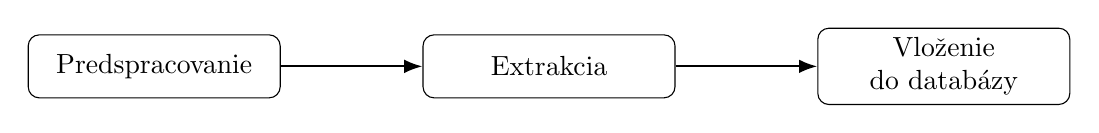
\begin{tikzpicture}[
  node distance=18mm,
  box/.style={draw, rounded corners, minimum height=8mm, minimum width=32mm, align=center},
  arr/.style={-Latex, thick}
]
  \node[box] (pre) {Predspracovanie};
  \node[box, right=of pre] (ext) {Extrakcia};
  \node[box, right=of ext] (db) {Vlo\v{z}enie\\do datab\'azy};

  \draw[arr] (pre) -- (ext);
  \draw[arr] (ext) -- (db);
\end{tikzpicture}
\end{center}


\subsection{Predspracovanie}
V tomto kroku sa PDF dokument načíta, klasifikuje a rozdelí na chunky. Dokument po načítaní
je klasifikovaný pomocou LLM Google Gemini-3-Flash, ktorý určí typ dokumentu (zmluva, zákon, vyhláška, atď.)
a do akého typu práva spadá (ústavné, finančné, občianske, atď.). Pre toto klasifikovanie využívam gemini, kvôli
jeho schopnosti spracovať veľké kontextové okná, rýchlosť ale taktiež pre najlepšie zosumarizovanie textu.
LLM posielam prvé dve strany dokumentu, system prompt, typy dokumentov a právnych odvetví,
a vzor na štruktúrovanú odpoveď.

\

Ako odpoveď dostanem objekt, kde je uložený typ dokumentu \texttt{type\textunderscore category} a typ právneho odvetvia \texttt{type\textunderscore legislation}.
V oboch pripádoch LLM musí uviesť percentuálnu istotu týchto údajov (v rozmedzí 0-100\%). K týmto údajom sa 
dá následne pristupovať ako k Python Dictionary.

\

V ďaľšom kroku prichádza na rozdelenie textu na časti. Využívam funkciu \textbf{RecursiveCharacterTextSplitter}
z balíku \texttt{langchain\textunderscore text\textunderscore splitters}. V otvorenej doméne na extrakciu
schémy rozdeľujem chunky s veľosťou 1200 tokenov a s prekrývaním 200 tokenov. Pri schéme-riadenom extrahovaní
su chunky nastavené na veľkosť 1024 tokenov s prekrývaním 128 tokenov.


\newpage
\subsection{Extrakcia}
Pri extrahovaní entít a vzťahov využívam hybridný prístup na extrakciu na základe štúdie tímu z
apple: \textbf{ODKE+: Ontology-Guided Open-Domain Knowledge Extraction with LLMs}. Kľúčovou vlastnosťou tohto
prístupu je využitie oboch prístupov: štruktúrovaného (schémov-riadené) a neštruktúrovaného (otvorená doména) extrahovania.

\

Prečo nie iba extrahovanie v otvorenej doméne? Po tomto prístupe by sme získali veľmi bohatý znalostný graf,
avšak s množstvom nekonzistentných údajov, duplicít a graf by bol chaotický. Kde by boli rozdielne typy entít
ako \texttt{Miesto} a \texttt{Lokácia}, a vznikala by fragmentácia.

\ 

Prečo nie iba schémov-riadené extrahovanie? Navrhnutie výstižnej a bohatej ontológie pre všetky typy práv je
časovo veľmi náročné. S najväčšou pravdepodobnosťou môže nastať situácia,
kde v nejakom dokumente sa vyskytne entita alebo vzťah, ktorý nie je definovaný v ontológii a je kľúčový
pre pochopenie dokumentu. Preto využívam kombináciu oboch prístupov. Je to časovo a cenovo neefektívne riešenie,
avšak prináša najlepšie výsledky. Presnosť extrahovania na základe štúdie dosahuje 98.8\%, čo je pre nás kľúčové.


\begin{center}
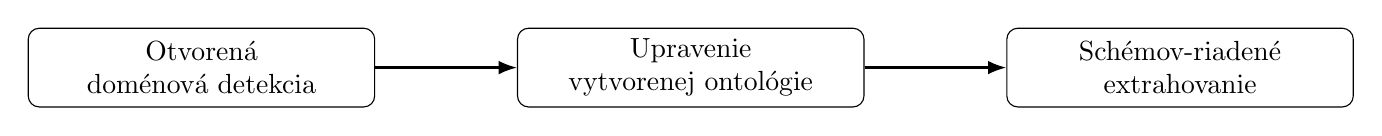
\begin{tikzpicture}[
  node distance=18mm,
  box/.style={draw, rounded corners, minimum height=10mm, minimum width=44mm, align=center},
  arr/.style={-Latex, thick}
]
  \node[box] (det) {Otvoren\'a\\dom\'enov\'a detekcia};
  \node[box, right=of det] (onto) {Upravenie\\vytvorenej ontol\'ogie};
  \node[box, right=of onto] (extr) {Sch\'emov-riaden\'e\\extrahovanie};

  \draw[arr] (det) -- (onto);
  \draw[arr] (onto) -- (extr);
\end{tikzpicture}
\end{center}

\subsubsection{Otvorená doménová detekcia}
Funkcia vytvorí z každého chunku proces, kde všetky procesy bežia paralelne na zníženie času spracovania.
V každom procese je volaný asynchrónne \texttt{agent}. Jehou úlohou je extrahovať každú jednu možnú entitu a vzťah,
ktoré sa nachádzajú v texte chunku. Je to z toho dôvodu, lebo tento krok odhalí nepreddefinované entity a vzťahy,
ktoré môžu byť kľúčové. Vďaka tomuto postupu sa ontológia dynamicky prispôsobí a rozšíri na klasifikovaný 
typ dokumentu a právneho odvetvia. Na tento účel využívam model gpt-4o pre jeho bohaté rozpoznávanie
textu. Následne je vrátená schéma ako zoznamy \texttt{list\textunderscore nodes}
a \texttt{list\textunderscore relationships}.

\subsubsection{Upravenie vytvorenej ontológie}
Vytvorená schéma z predchádzajúceho kroku je poslaná na upravenie. LLM porovná schému s 
preddefinovanou vzorovou ontológiou (sada vytvorených ontológií, ktoré sú konzistentné naprieč slovenským
právom napr. \texttt{Osoba}, \texttt{Zákon}, \texttt{Paragraf}, ...) alebo s už existujúcou schémou znalostného grafu. Tento krok je dôležitý, aby boli údaje
konzistentné, nevytvárali sa sémanticky podobné entity a vzťahy (napr. \texttt{UPRAVUJE} vs \texttt{UPRAVIL})
a nevznikali duplicity. Výstupom tohto kroku je upravená schéma ako zoznamy \texttt{nodes} a \texttt{relationships}.
Využívaný model je gemini-3-flash kvôli jeho dobrým schopnostiam rozmýšľať a odvôvodniť.

\

\subsubsection{Schémov-riadené extrahovanie}
Najprecíznejší krok extrakcie, ktorý zaručuje najvyššiu presnosť a kvalitu extrakcie. Tak isto ako v
otvorenej doméne, aj tu je každý chunk je spracovaný paralelne.
LLM je poskytnutá ontológia z predošlého kroku a na jej základe extrahuje konzistentné entity a vzťahy.
\texttt{Agent} vráti zoznamy \texttt{nodes} a \texttt{relationships}, ktoré sú následne transformované
do \texttt{GraphDocument} objektu.


\ 

Výsledkom je bohatý, konzistentný znalostný graf, ktorý obsahuje všetky relevantné informácie z právnych dokumentov.
Chunky a dokumenty sú pospájané pomocou vzťahu \texttt{IN\textunderscore DOCUMENT} a chunky s entitami pomocou vzťahu
\texttt{HAS\textunderscore ENTITY}. Medzi entitami sú vzťahy, ktoré sú extrahované z dokumentu.

\

\begin{center}
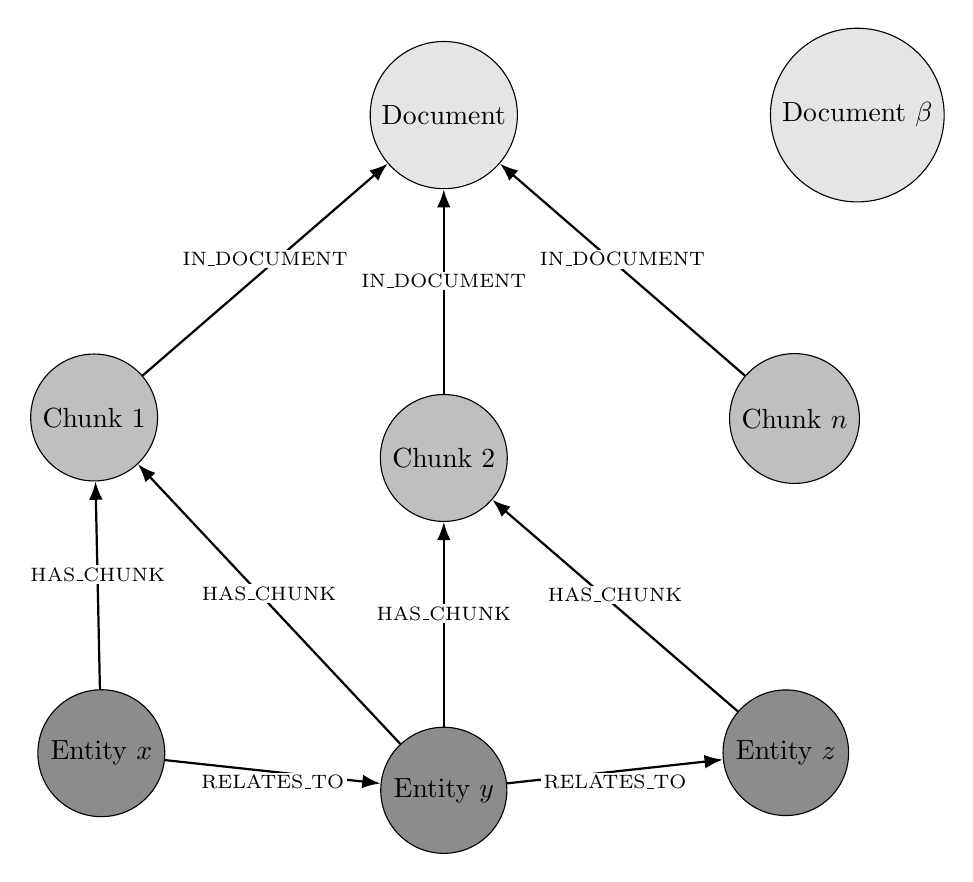
\begin{tikzpicture}[
  node distance=26mm and 32mm,
  doc/.style={circle, draw, fill=gray!20, minimum size=14mm, align=center},
  chunk/.style={circle, draw, fill=gray!50, minimum size=14mm, align=center},
  ent/.style={circle, draw, fill=gray!90, minimum size=14mm, align=center},
  arr/.style={-Latex, thick}
]

  \node[doc] (doc) {Document};
  \node[doc, right=of doc] (doc2) {Document $\beta$};

  \node[chunk, below left=of doc] (c1) {Chunk 1};
  \node[chunk, below=of doc] (c2) {Chunk 2};
  \node[chunk, below right=of doc] (cn) {Chunk $n$};

  \node[ent, below left=of c2] (ex) {Entity $x$};
  \node[ent, below=of c2] (ey) {Entity $y$};
  \node[ent, below right=of c2] (ez) {Entity $z$};

  \draw[arr] (c1) -- node[midway, above, fill=white, inner sep=1pt]{\scriptsize IN\_DOCUMENT} (doc);
  \draw[arr] (c2) -- node[midway, above, fill=white, inner sep=1pt]{\scriptsize IN\_DOCUMENT} (doc);
  \draw[arr] (cn) -- node[midway, above, fill=white, inner sep=1pt]{\scriptsize IN\_DOCUMENT} (doc);

  \draw[arr] (ex) -- node[midway, above, fill=white, inner sep=1pt]{\scriptsize HAS\_CHUNK} (c1);
  \draw[arr] (ey) -- node[midway, above, fill=white, inner sep=1pt]{\scriptsize HAS\_CHUNK} (c1);
  \draw[arr] (ey) -- node[midway, above, fill=white, inner sep=1pt]{\scriptsize HAS\_CHUNK} (c2);
  \draw[arr] (ez) -- node[midway, above, fill=white, inner sep=1pt]{\scriptsize HAS\_CHUNK} (c2);

  \draw[arr] (ex) -- node[midway, below, fill=white, inner sep=1pt]{\scriptsize RELATES\_TO} (ey);
  \draw[arr] (ey) -- node[midway, below, fill=white, inner sep=1pt]{\scriptsize RELATES\_TO} (ez);
\end{tikzpicture}
\end{center}


\newpage
\subsection{Vkladanie do databázy}
Údaje vkladáme do dvoch typov databáz: grafovej databázy Neo4j a vektorovej databázy Neo4jVector.

\

\noindent\textbf{Grafová databáza}
\ 

Do grafovej databázy vkladáme \texttt{GraphDocument}. Na úspešne vloženie je potrebné si doinštalovať
do inštancie \textbf{APOC plugin} cez Neo4j Desktop aplikáciu.

\

\noindent Úkažka \texttt{GraphDocument}:
{\scriptsize
\begin{verbatim}
{
    "nodes": [
      {
        "id": "POŽIADAVKY NA BEZPEČNOSTNÝ RIADIACI SYSTÉM",
        "type": "Document",
        "properties": {
          "name": "POŽIADAVKY NA BEZPEČNOSTNÝ RIADIACI SYSTÉM"
        }
      },
      {
        "id": "Organizačná štruktúra podniku",
        "type": "Organizational_structure",
        "properties": {
          "name": "Organizačná štruktúra podniku"
        }
      },
      ... ,
      {
        "id": "chunk_0",
        "type": "Chunk",
        "properties": {
          "text": "25 \n \n \nPOŽIADAVKY NA BEZPEČNOSTNÝ RIADIACI SYSTÉM \n ...",
          "embedding": [
            0.013147621415555477,
            -0.027107400819659233,
            0.005099280271679163,
            ...
          ]
        }
      }
    ],
    "relationships": [
      {
        "source_id": "POŽIADAVKY NA BEZPEČNOSTNÝ RIADIACI SYSTÉM",
        "source_type": "Document",
        "relation": "CONTAINS",
        "target_id": "Organizačná štruktúra podniku",
        "target_type": "Organizational_structure",
        "properties": {}
      },
      {
        "source_id": "Organizačná štruktúra podniku",
        "source_type": "Organizational_structure",
        "relation": "INCLUDES",
        "target_id": "zamestnanci",
        "target_type": "Employee",
        "properties": {}
      },
      ...
    ],
    "source": {

    }
}
\end{verbatim}
}
{\scriptsize * \textit{... znamená že text pokračuje ďalej alebo existujú ďaľšie entity a vzťahy}}

\newpage
V grafovej databáze majú údaje podobnú štruktúru ako v \texttt{GraphDocument}. Pri \texttt{nodes}, má
každá entita svoj unikátny \texttt{elementId}, \texttt{labels} (štítok alebo typ v Neo4j), kde
každý \texttt{node} má typ \textunderscore\textunderscore Entity\textunderscore\textunderscore a svoj vlastný typ, 
a \texttt{properties}. Pri \texttt{relationships} je \texttt{type}, \texttt{elementId}, \texttt{startNodeElementId} a
\texttt{endNodeElementId}.

\begin{figure}[h]
  \centering
  \begin{subfigure}[c]{0.45\textwidth}
    \centering
    \includegraphics[width=\textwidth]{../legal_graph.png}
    \caption{Grafová databáza so zobrazenými entitami a vzťahmi}
    \label{fig:legal_graph}
  \end{subfigure}
  \hfill
  \begin{subfigure}[c]{0.45\textwidth}
    \centering
    \includegraphics[width=\textwidth]{../legal_graph_data.png}
    \caption{Grafová databáza so dátami}
    \label{fig:legal_graph_data}
  \end{subfigure}
\end{figure}



\

\noindent\textbf{Vektorová databáza}
\

Do vektorovej databázy vkladáme embeddingy entít a vzťahov. Tieto embeddingy sú využívané na rýchlejšie
sémantické vyhľadávanie. Vektorová databáza je prepojená s grafovou databázou cez unikátne \texttt{elementId}.
Výsledky sa vyhľadávajú pomocou podobnosti vektorov a ich kosínusovej vzdialenosti.


\

\section{Vyhľadávanie}
Na vyhľadávanie respektíve na zodpovedanie otázky od používateľa, využívam metódu hybridný GraphRAG (Graph Retrieval-Augmented Generation).
Je to kombinácia dvoch prístupov: vyhľadávanie v znalostnom grafe a sémantické vyhľadávanie pomocou vektorovej databázy.

\ 

Následujúci graf zobrazuje jednotlivé kroky, pri hľadaní odpovede na otázku od používateľa:

\begin{center}
\resizebox{\linewidth}{!}{
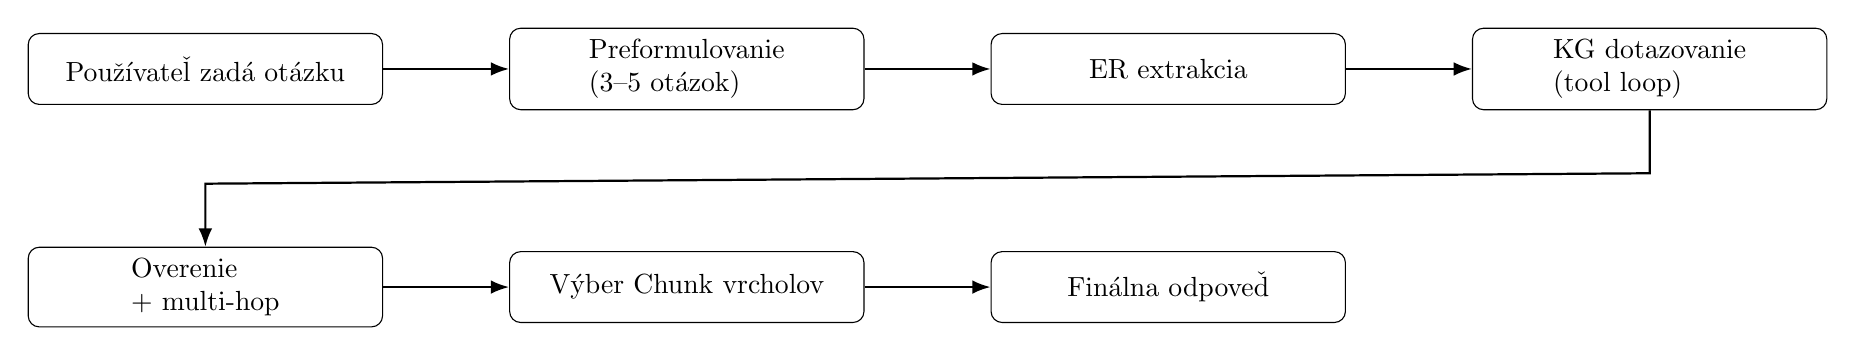
\begin{tikzpicture}[
  node distance=14mm and 16mm,
  box/.style={draw, rounded corners, align=left, minimum width=45mm, minimum height=9mm, inner sep=4pt},
  arr/.style={-Latex, thick}
]
  % 1st row
  \node[box] (uq) {Používateľ zadá otázku};
  \node[box, right=of uq] (rq) {Preformulovanie\\(3--5 otázok)};
  \node[box, right=of rq] (svo) {ER extrakcia};
  \node[box, right=of svo] (kg) {KG dotazovanie\\(tool loop)};

  % 2nd row (wrap)
  \node[box, below=18mm of uq] (mh) {Overenie \\+ multi-hop};
  \node[box, right=of mh] (ch) {Výber Chunk vrcholov};
  \node[box, right=of ch] (ans) {Finálna odpoveď};

  \draw[arr] (uq) -- (rq);
  \draw[arr] (rq) -- (svo);
  \draw[arr] (svo) -- (kg);

  \draw[arr] (kg.south) -- ++(0,-8mm) -- ($(mh.north)+(0,8mm)$) -- (mh.north);
  \draw[arr] (mh) -- (ch);
  \draw[arr] (ch) -- (ans);
\end{tikzpicture}
}
\end{center}

\subsection{Používateľ zadá otázku}
Používateľ zadá otázku v prirodzenom jazyku, prostredníctvom metódy \texttt{graphrag.query}.
\begin{lstlisting}
graphrag.query(user_question)
\end{lstlisting}

\subsection{Preformulovanie}
LLM vytvorí 3-5 preformulovaných otázok. V každej jednej otázke sa snaží zahrnúť kľúčové informácie z 
pôvodnej otázky, ale formulované iným spôsobom. Cieľom je získať rôzne pohľady na otázku, aby sme 
maximalizovali šancu na získanie relevantných informácií z grafovej databázy.

\subsection{ER extrakcia}
Pre každú preformulovanú otázku, LLM extrahuje entity a vzťahy. Využíva sa extrakcia na otvorenej doméne,
kde sa neberie ohľad na typ entít a vzťahov, ale extrahujú sa všetky možné entity a vzťahy, ktoré sa 
nachádzajú v otázke. Tieto entity a vzťahy sú následne použité na dotazovanie sa do grafovej databázy.

\subsection{KG dotazovanie}
Pre každú entitu a vzťah sa nájdu entity a vzťahy vo vektorovej databáze na základe sémantickej podobnosti.
Tieto entity a vzťahy sú prepojené s grafovou databázou cez \texttt{elementId}.
Následne pomocou týchto entít a vzťahov, LLM vytvorí Cypher Query, ktoré sa použije na dotazovanie 
do grafovej databázy. Tento krok je iteratívny, kde LLM môže vytvoriť viacero dotazov, 
ktoré sa postupne spúšťajú, pomocou nástroja, ktorý ma obmedzený prístup do databázy. 
Výsledky z týchto dotazov sú následne použité na overenie a multi-hop vyhľadávanie.

\subsection{Overenie + multi-hop}
Tento krok predstavuje kontrolný mechanizmus a logické jadro vyhľadávacieho procesu. LLM analyzuje 
výsledky získané z predchádzajúcich grafových dopytov a posudzuje ich relevanciu vzhľadom na komplexnosť 
právneho problému.

\

Ak sú získané informácie fragmentované alebo neúplné, aktivuje sa multi-hop reasoning. Tento proces 
umožňuje systému: 
\begin{itemize} 
    \item \textbf{Prechádzanie relácií:} Identifikovať prepojenia medzi 
    entitami, ktoré nie sú v priamom vzťahu (napr. prepojenie konkrétnej osoby cez zmluvu až k príslušnému 
    zákonu). 
    \item \textbf{Dopĺňanie kontextu:} Ak odpoveď vyžaduje informáciu z inej časti grafu, model 
    iniciuje ďalšiu iteráciu dopytovania na základe novoobjavených uzlov. 
    \item \textbf{Eliminácia halucinácií:} Overením faktov priamo voči štruktúre grafu sa zabezpečí, 
    že výsledná odpoveď bude podložená reálnymi vzťahmi v legislatívnom dokumente, nie len 
    pravdepodobnostným odhadom modelu. 
\end{itemize}

\noindent Výsledkom je overený vedomostný základ, ktorý slúži ako presný podklad pre finálnu syntézu odpovede.

\subsection{Výber Chunk vrcholov}
Pre všetky nájdené vrcholy z grafu vrátime pomocou vzťahu \texttt{HAS\textunderscore CHUNK} vrcholy Chunk a ich atribút s textom.

\subsection{Finálna odpoveď}
Výsledná odpoveď je vytvorená z:
\begin{itemize}
    \item pôvodnej otázky od používateľa,
    \item preformulovaných otázok,
    \item znalostných grafov,
    \item textu z Chunk vrcholov,
    \item System prompt.
\end{itemize}

\noindent Tieto informácie sú poskytnuté Gemini, ktorý vďaka jeho veľkému kontextovému oknu, dokáže spracovať údaje
a odpovedať na otázku.




\section{Testovanie a výsledky}
Testovanie systému bolo robené na knihe \textbf{Romeo a Júlia}, kde bolo otestované spracovanie knihy a vyhľadávanie.

\

Prvotné spracovanie knihy bolo robené na otvorenej doméne, kde sa extrahovali všetky možné entity a vzťahy. Toto
riešenie prinieslo bohatý graf, avšak chýbala konzistencia. Následne bolo testované schémov-riadené extrahovanie, 
kde sa použila mnou upravená schéma z otvorenej domény. Toto riešenie prinieslo konzistentný graf a počet 
entít bol približne rovnaký ako v otvorenej doméne: $N_{oe} = 2536 \approx N_{sde} = 2512$. Taktiež bolo 
upravené spracovanie zo synchrónneho na asynchrónne, čo znížilo čas spracovania pri tejto knihe
približne \textit{6x}: $T_{sync} = 12min \approx T_{async} = 2min$.

\

Na overenie spracovania grafu a relevantnosti údajov, som vytvoril agenta na iteratívne dotazovanie databázy.
Tento agent má obmedzený prístup do grafovej databázy, kde pomocou nástroja môže spúšťať Cypher Queries a upravovať
ich podľa vrátených údajov. Pri tomto vyhľadávaní bol čas spracovávania v rozmedzí \textit{20 sekúnd} až \textit{4 minúty}.
Problém je v jeho neobmedzenosti a hľadania do posledného detailu. Relevantné údaje však vždy našiel a odpoveď bola 
vďaka týmto údajom vždy presná a správna. 

Príklad vytvorenej Cypher Query na otázku \textit{"Which Characters who belong to the Capulet house are in love with a Character who belongs to the Montague house?"}:

{\scriptsize
\begin{verbatim}
    MATCH (cap)-[b:BELONGS_TO]-(h:House)\nWHERE toLower(h.id) CONTAINS toLower('capulet') AND 
    (cap:Character OR cap:Person)\nMATCH (cap)-[r]-(m)\nWHERE type(r) IN ['LOVES','IN_LOVE_WITH','LOVE',
    'EXPRESSES_FEELING_FOR','TENDER_LOVE','POTENTIAL_LOVE','WOO','LOVER'] AND (m:Character OR m:Person)\nMATCH 
    (m)-[bm:BELONGS_TO]-(h2:House)\nWHERE toLower(h2.id) CONTAINS toLower('montague')\nRETURN DISTINCT cap.id AS 
    capulet_character, labels(cap) AS capulet_labels, type(r) AS rel_type, m.id AS montague_character, labels(m) AS 
    montague_labels, properties(cap) AS cap_props, properties(m) AS mont_props\nLIMIT 25
\end{verbatim}
}

\noindent Vrátené údaje z tejto query:
{\scriptsize
\begin{verbatim}
    "nodes_found": [
            "Juliet",
            "Romeo",
            "Capulet",
            "Montague"
          ],
          "relationships_found": [
            "Juliet -[LOVES]-> Romeo",
            "Juliet -[EXPRESSES_FEELING_FOR]-> Romeo",
            "Juliet -[LOVER]-> Romeo",
            "Juliet -[LOVE]-> Romeo",
            "Juliet -[IN_LOVE_WITH]-> Romeo",
            "Juliet -[BELONGS_TO]-> Capulet",
            "Romeo -[BELONGS_TO]-> Montague"
          ]
        },
\end{verbatim}
}

\noindent Tu vidíme nekonzistentnosť vzťahov v otvorenej doméne. Namiesto jedného vzťahu
\texttt{LOVES} máme päť. Na základe týchto údajov odpoveď bola správna: \texttt{Juliet}.
Spracovanie na tejto knihe pomohlo upresniť a vylepšiť systém. Overovať kvalitu údajov bolo
veľmi jednoduché a presné, čo by sa na zbierke zákona robilo veľmi obtiažne.

\      

Následne som začal s implementáciou hybridného spracovania pre legálne dokumenty.
Tu testujem spracovanie na dokumentoch zo zbierky zákona. Ako zdroj dokuemntov používam: \url{https://www.slov-lex.sk}.
Dokumenty sa dajú vyhľadávať podľa odvetvia práva a typu dokumentu.



\section{Plán na letný semester}
\begin{itemize}
    \item Dokončiť implementáciu vyhľadávania a multi-hopu
    \item Optimalizácia promptov pre rýchlejšie spracovanie a vyhľadávanie
    \item Vytvorenie používateľského rozhrania (webová aplikácia) pre jednoduché zadávanie otázok, zobrazenie nájdených znalostných grafov a zobrazovanie odpovedí.
\end{itemize}   

\end{document}